\section{6FLAS: Lightweight Security Mechanism}
\label{sec:method}

This section presents 6FLAS. The two design principles that motivate the
mechanism are introduced first, followed by its two cooperating carriers: a
Flow-Label-based stateless flow authenticator and an SRv6-integrated security
segment that drives constant-time per-hop verification. Domain key management
and an end-to-end walk-through of the data path conclude the section. Throughout, the design keeps a single invariant in view: the only mutable on-board state is a small
per-direction replay window, never anything per flow.
\cref{fig:arch} shows the overall architecture.

\begin{figure}[t]
\centering
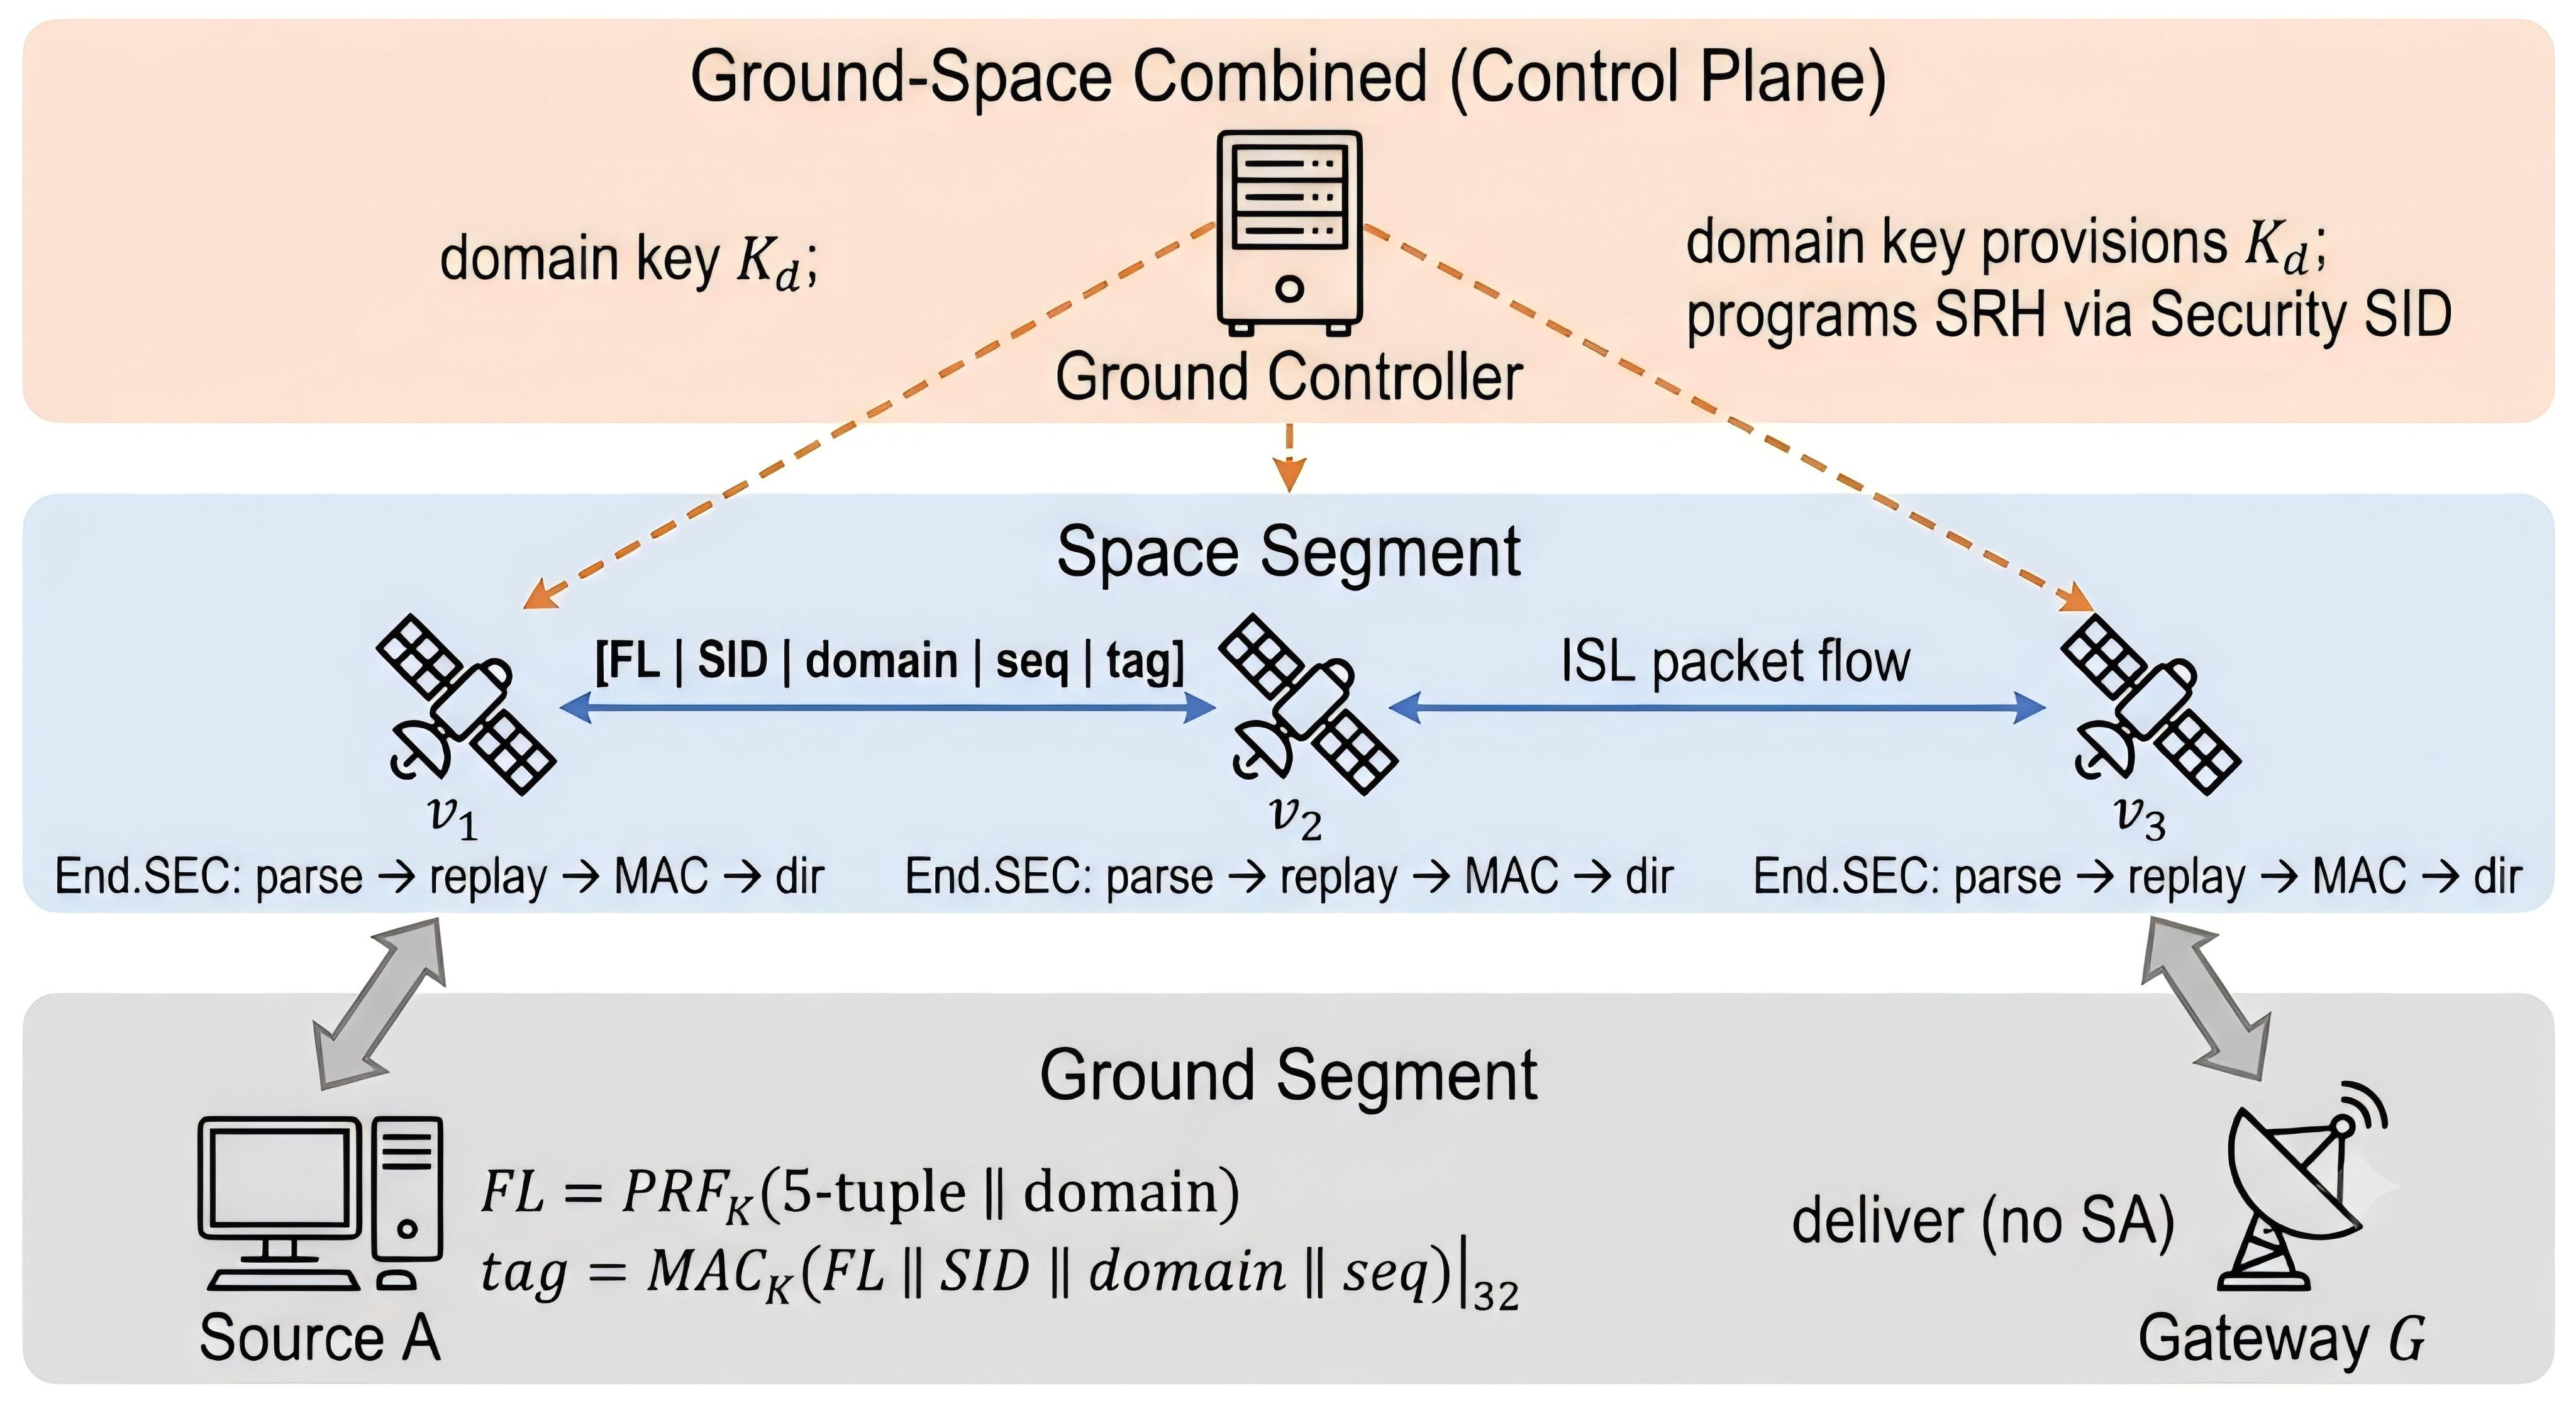
\includegraphics[width=\columnwidth]{figures/arch.jpg}
\caption{6FLAS three-segment architecture.
\textit{Ground segment}: source $A$ computes the Flow Label
$\fl=\prf_{\skey_\domid}(\textit{5-tuple}\,\|\,\domid)$ and the 32-bit MAC tag
before transmission; gateway $G$ delivers packets with no per-flow SA.
\textit{Space segment}: each on-board router executes the four-step
\texttt{End.SEC} procedure (\cref{alg:verify}) over ISLs — no per-flow state
migrates on handover.
\textit{Ground-space combined (control plane)}: the ground controller provisions
domain key $\skey_\domid$ to all nodes and programs the SRH path via Security SIDs;
bidirectional arrows denote space-ground uplinks.}
\label{fig:arch}
\end{figure}

\subsection{Design Philosophy}
\label{sec:philosophy}

6FLAS rests on two ideas. First, \emph{carry security state in the packet, not on
the satellite}. A stateful protocol stores a security association per flow at
every protected node; 6FLAS instead derives a compact authenticator from a
domain key and embeds it in fields the packet already carries, so a verifying
router needs no per-flow record. This drives the per-flow state term
$m_{\mathcal{M}}$ in \cref{eq:feasibility} toward zero and makes the mechanism
indifferent to ISL handovers: when a flow is rerouted, no SA migrates because
none exists. Second, \emph{exploit the structured LEO topology}. Because each
router forwards over a small fixed set of grid directions
(\cref{sec:leo-char}), the egress access-control check, which on a general
router needs a routing/policy lookup, becomes a constant-time comparison
against the SID-encoded expected direction.

The two carriers are complementary. The immutable, source-set Flow Label
(\cref{sec:fl-srv6}) supplies a stable, source-bound flow-identity token that is
the same at every hop; the SRv6 Security SID supplies the per-hop path policy
and the bytes over which integrity is checked. \cref{fig:overview} shows the
resulting packet and the per-hop pipeline.

\begin{figure}[t]
\centering
\footnotesize
\setlength{\fboxsep}{4pt}
\fbox{\parbox{\dimexpr\columnwidth-2\fboxsep-2\fboxrule\relax}{\centering
\textbf{IPv6 base header} \;[\,\textbf{Flow Label} $\fl$ = $\prf_{\skey_\domid}(\text{5-tuple}\,\|\,\domid)$\,] \\[2pt]
$\downarrow$ \\[2pt]
\textbf{SRH} \;[\,Segment list $\;\dots\;$ \textbf{Security SID} = Loc$\,|\,$Func$\,|\,$Args\,] \\[2pt]
$\downarrow$ \\[2pt]
\textbf{6FLAS metadata (8\,B)}: \;[\,domain $\domid$ | seq $\seq$ | tag $\mtag$\,] \\[2pt]
$\downarrow$ \\[2pt]
\textbf{Payload} (optionally encrypted, out of scope)
}}
\caption{6FLAS packet structure. The Flow Label carries a stateless flow
authenticator; the SRv6 Security SID encodes the per-hop path policy; an
8-byte metadata block carries the domain id, sequence number, and truncated MAC
tag. Each on-board router verifies the tag over the covered routing span and
checks the replay window, then forwards.}
\label{fig:overview}
\end{figure}

\subsection{Flow-Label-Based Stream Authentication}
\label{sec:fl-auth}

\begin{definition}[Authenticated flow]
\label{def:flow}
A 6FLAS flow is the tuple $f=(\textsf{5tuple},\domid)$ where \textsf{5tuple} is
the IPv6 five-tuple (source/destination address, source/destination port,
next-header) and $\domid$ is a security-domain identifier shared by the
authorized routers serving the flow.
\end{definition}

The source node sets the Flow Label deterministically from the flow and the
domain key $\skey_\domid$:
\begin{equation}
\label{eq:fl}
\fl \;=\; \prf_{\skey_\domid}(\textsf{5tuple}\,\|\,\domid) \bmod 2^{20},
\end{equation}
where $\prf$ is a keyed pseudorandom function (using a SipHash-class keyed
PRF~\cite{siphash}). By RFC~6437 the label is then immutable in
transit~\cite{rfc6437}, so $\fl$ is a stable, source-bound token that every hop
observes identically. Because $\skey_\domid$ is secret, an off-path adversary
cannot compute the label that a given five-tuple should carry, and an on-path
adversary that copies $\fl$ cannot reuse it for a different five-tuple without
detection (the per-packet MAC below binds them together). The 20-bit space
admits up to $2^{20}\approx 1.05$M concurrent labels per domain; collision
behavior under heavy load is discussed in the evaluation.

Each packet carries an 8-byte 6FLAS metadata block: a 1-byte domain id $\domid$,
a 3-byte monotonically increasing sequence number $\seq$, and a 4-byte
truncated MAC tag
\begin{equation}
\label{eq:tag}
\mtag \;=\; \mac_{\skey_\domid}\!\bigl(\fl \,\|\, \textsf{SID} \,\|\, \domid \,\|\, \seq\bigr)\big|_{32},
\end{equation}
computed over the immutable Flow Label, the active Security SID, the domain id,
and the sequence number. A verifying router recomputes \cref{eq:tag} from
fields already in the packet plus the domain key it holds; no per-flow state is
consulted. The tag binds the flow identity ($\fl$), the path policy
(\textsf{SID}), and the freshness ($\seq$) together, so altering any of them
invalidates the tag (R1, R2). \cref{sec:security} bounds the forgery
probability of the 32-bit truncation.

The 3-byte sequence counter $\seq$ resets on each transport-level reconnection,
and domain-key rotation implicitly invalidates old counters, so rollover is not
a concern in normal operation. The per-direction replay window $W_v$ uses a
$w=256$-entry bitmap (32\,B per direction), giving a total on-board state of
$6\times32=192$\,bytes for the six $+$Grid directions — independent of the flow
count and well within any space-grade processor's memory budget.

\subsection{SRv6 Security Segment and Per-Hop Verification}
\label{sec:srv6-bind}

6FLAS encodes its per-hop policy in an SRv6 Security SID that follows the
standard \texttt{Locator$\,|\,$Function$\,|\,$Arguments} layout~\cite{rfc8986}.
The \texttt{End.SEC} function is defined as a strict superset of \texttt{End},
so nodes that implement only \texttt{End} continue forwarding without
interruption.

\begin{definition}[Security SID behavior \texttt{End.SEC}]
\label{def:endsec}
When a router $v$ receives a packet whose active SID carries the \texttt{End.SEC}
function code, it executes \cref{alg:verify} before performing the standard
SRv6 \texttt{End}/\texttt{End.X} forwarding action. If any check in
\cref{alg:verify} fails, the packet is dropped and no SRv6 processing occurs.
If all checks pass, $v$ advances the Segments Left pointer, applies the standard
SRv6 forwarding action for the next SID, and advances the replay window. A node
that implements \texttt{End} but not \texttt{End.SEC} performs standard
\texttt{End}/\texttt{End.X} forwarding without the security checks, interoperating
with the overlay but providing no per-hop verification.
\end{definition}

\begin{itemize}
    \item \textbf{Locator} (64\,b): routes the packet toward the next 6FLAS node,
    exactly as in standard SRv6.
    \item \textbf{Function} (16\,b): a code point \texttt{End.SEC} that triggers
    6FLAS verification before the usual \texttt{End}/\texttt{End.X} forwarding.
    \item \textbf{Arguments} (48\,b): the path security policy, encoding the
    expected ingress direction, the authorized egress direction (one of the six
    fixed LEO grid directions), and a domain/policy tag matched against $\domid$.
\end{itemize}

Encoding the expected egress direction in the SID is what lets a router enforce
access control (R4) without a routing-table or policy lookup: the controller
that programs the path writes the intended next direction into the SID at
source time, and each hop simply checks that its actual forwarding direction
matches. \cref{tab:args} shows the 48-bit Arguments field layout.

\begin{table}[t]
\centering
\caption{6FLAS Security SID Arguments field (48 bits total).}
\label{tab:args}
\renewcommand{\arraystretch}{1.2}
\begin{tabular}{lrl}
\toprule
\textbf{Field} & \textbf{Bits} & \textbf{Description} \\
\midrule
Ingress dir.   & 4  & Expected ingress dir.\ (3\,b index + 1\,b reserved) \\
Egress dir.    & 4  & Authorized egress dir.\ (3\,b index + 1\,b reserved) \\
Domain id      & 8  & Matches $\domid$ in 6FLAS metadata block \\
Path-policy    & 32 & Controller-set policy hash for the flow group \\
\bottomrule
\end{tabular}
\end{table}

\paragraph{Per-hop verification}
\label{sec:perhop}
\cref{alg:verify} gives the per-hop procedure. After parsing the IPv6 base
header and the active SID, the router (1) hashes the Flow Label into a small
per-direction replay-window table to locate the relevant window in $O(1)$,
(2) checks the sequence number against the sliding window for anti-replay (R3),
(3) recomputes the MAC of \cref{eq:tag} and compares it in constant time to the
carried tag (R1, R2), and (4) checks that the SID-encoded egress direction is
one of the node's authorized directions before forwarding (R4). Every step uses
only fields in the packet and the domain key; there is no per-flow SA lookup.

\begin{algorithm}[t]
\caption{6FLAS per-hop verification at router $v$}
\label{alg:verify}
\begin{algorithmic}[1]
\Require packet $p$; domain keys $\{\skey_\domid\}$; replay windows $W_v[\,\cdot\,]$
\State $(\fl,\textsf{SID},\domid,\seq,\mtag) \gets \textsc{Parse}(p)$
\If{$\domid \notin$ authorized domains at $v$} \State \textbf{drop} \EndIf
\State $w \gets W_v[\,\textsf{hash}(\fl)\ \%\ |W_v|\,]$ \Comment{$O(1)$ window select}
\If{$\seq \le w.\text{base}$ \textbf{or} $w.\text{seen}(\seq)$}
    \State \textbf{drop} \Comment{replayed / stale (R3)}
\EndIf
\State $\mtag' \gets \mac_{\skey_\domid}(\fl \,\|\, \textsf{SID} \,\|\, \domid \,\|\, \seq)\big|_{32}$
\If{$\mtag' \neq \mtag$} \State \textbf{drop} \Comment{forged / tampered (R1,R2)} \EndIf
\State $\text{dir} \gets \textsc{Egress}(\textsf{SID.Args})$
\If{$\text{dir} \notin$ authorized directions at $v$}
    \State \textbf{drop} \Comment{policy violation (R4)}
\EndIf
\State $w.\textsc{Advance}(\seq)$; \quad \textsc{ApplySRv6}(p); \quad \textbf{forward}
\end{algorithmic}
\end{algorithm}

\paragraph{Topology-aware optimization and statelessness.}
A general router enforcing an egress policy would consult a forwarding or
policy table whose size grows with the number of destinations. In a $+$Grid LEO
node the authorized egress set has at most six members (north/south intra-plane,
east/west inter-plane, up/down ground), so line~11 of \cref{alg:verify} is a
comparison against a six-element fixed set, i.e., constant time and constant
space, independent of $|\setF|$. Likewise the replay window table $W_v$ is sized
per direction, not per flow, so its memory is $O(1)$ in the flow count. These
specializations are what make 6FLAS satisfy the feasibility condition
\cref{eq:feasibility} at $10^6$ flows where stateful schemes do not. The only
mutable state a 6FLAS router keeps is the bounded per-direction replay window
$W_v$, independent of the number of flows: many flows hash into the same window,
and the window only tracks recently seen sequence numbers within a time horizon.
Thus $m_{\mathcal{M}}$ per flow is effectively zero, and
a handover that reroutes a flow requires no state transfer, directly satisfying
D2 and D3.

\paragraph{Hardware pipeline mapping.}
\cref{alg:verify} decomposes into four stages with no inter-stage feedback:
(1)~header parse and domain-id gate, (2)~replay-window probe,
(3)~MAC recompute, and (4)~direction check and window advance.
Stages~2 and~4 access only the 192-byte on-chip SRAM described above; stage~3
feeds the keyed-MAC core directly from parsed header fields with no memory
indirection. Because stage~3 is the critical-path stage (${\approx}306$\,ns at
1\,GHz), throughput is limited by the MAC core rather than any data-dependent
memory access, and a pipelined implementation sustains one verification per
MAC-core cycle. This pipeline structure is exactly what makes 6FLAS amenable
to FPGA or ASIC realization on a space-grade logic fabric~\cite{li2022}: the
critical path is a fixed-width keyed-hash, and the only state written back per
packet is a single bit in the 192-byte replay bitmap.

\subsection{Domain Key Management}
\label{sec:keymgmt}

6FLAS verification requires each authorized router to hold the domain key
$\skey_\domid$; a full key-management protocol is out of scope~\cite{tan2025crossdomain},
but the stateless design keeps the overhead light. The domain key is a symmetric
secret shared among all nodes in domain $\domid$; large constellations partition
into multiple domains (up to 256 via the 1-byte $\domid$ field) to bound the
blast radius of a compromise. Each satellite is provisioned at manufacture or via
a secured telecommand channel with the keys of the domains it serves.
Ground terminals acting as packet sources are similarly provisioned through
the same ground-based key-management channel, since computing $\fl$
(\cref{eq:fl}) and the initial tag (\cref{eq:tag}) both require $\skey_\domid$;
the security perimeter of a domain thus spans all authorized senders and
verifiers sharing $\skey_\domid$. Rotation
follows an epoch schedule: the operator pushes $\skey_{\domid}^{(e+1)}$ to all
nodes before epoch $e{+}1$ begins; verifiers accept both the current and the
immediately previous epoch to absorb in-flight packets. Because updates are
domain-granular, bandwidth scales as $O(|D|)$, not $O(|\setF|)$ — for 256
domains with 128-bit keys, each epoch push is only $4096$\,bytes. Revocation
rotates the affected domain key and immediately invalidates any traffic an
adversary could mint; because 6FLAS holds no per-flow secrets, revocation
granularity is the domain, which is coarse but cheap.

To make the data path concrete, consider a packet from source $A$ to gateway $G$
routed through three on-board nodes $v_1{\to}v_2{\to}v_3$ in domain
$\domid{=}7$. At the source, $A$ computes
$\fl=\prf_{\skey_7}(\textsf{5tuple}\,\|\,7)\bmod 2^{20}$, writes it into the
IPv6 Flow Label, pushes an SRH whose active Security SID at each hop encodes the
intended egress direction (e.g., \texttt{east}, \texttt{north}, \texttt{down}),
sets $\seq$ from its per-flow counter, and computes the $32$-bit tag
$\mtag=\mac_{\skey_7}(\fl\,\|\,\textsf{SID}\,\|\,7\,\|\,\seq)|_{32}$. At $v_1$,
the router reads $\domid{=}7$ (authorized), selects the replay window by
$\textsf{hash}(\fl)$, checks $\seq$, recomputes the tag over the same span and
matches it, confirms its egress is \texttt{east}, advances the window, and
forwards. Nodes $v_2$ and $v_3$ repeat the identical $O(1)$ check against their
own authorized directions. No node ever created, looked up, or migrated a
per-flow record; if an ISL break reroutes the flow through a different $v_2'$,
that node verifies the next packet with $\skey_7$ exactly as $v_2$ would have,
with no re-keying.
